\documentclass[titlepage,11pt,a4paper]{article}
\usepackage[utf8]{inputenc} \usepackage[english]{babel}

% I think these margin options are quite nice
\usepackage[top=1in, bottom=1.25in, left=1.25in,
  right=1.25in]{geometry}

\usepackage{graphicx} \usepackage{float}
\PassOptionsToPackage{hyphens}{url}\usepackage[hidelinks]{hyperref}

\hypersetup{ pdfinfo={ Author={SML}, Title={Developer's Guide},
    Creator={LaTeX} } }

\title{Developer's Guide} \author{SML}


\begin{document}
\maketitle \tableofcontents
\newpage

\section{Introduction}
% Short about our project 
This document describes the different parts of the program for
quadcopters developed on the Access Summer Project, 2015, and before,
in the Smart Mobility Lab, KTH.

% The hardware that we used 
The quadcopters used, and for which this guide is aimed, are the 3DR
IRIS$^+$. As a motion capture system Qualisys was used. The
quadcopters use the Pixhawk autopilot. For changing settings of the
quadcopters the program Mission Planner, version XXX, was used,
\url{http://planner.ardupilot.com/}. Most parts of the code is written
in Python.

% About this guide
This guide provide information about how the program is structured,
Sec.~\ref{sec:architecture}, how ...


\section{Architecture}
\label{sec:architecture}

\begin{figure}[h!]                                                               
  \centering \includegraphics[width=\textwidth]{figures/architecture}
  \caption{The architecture used in ROS. Only main parts and
    connections in shown. X $= 1, 2, 3, \dots$}
  \label{fig:architecture}                                                              
\end{figure}

The program is using ROS, \textit{The Robot Operating System}, to
connect different parts of the program. A basic knowledge of ROS is
assumed. The architecture used in the program is shown in
Fig.~\ref{fig:architecture}. Circles does not correspond to ROS nodes
strictly, but describes the different parts of the
program. Rectangles, however, correspond to ROS topics. ROS packages
are also written in the figure. Arrows with black head corresponds to
publication to a topic, if the arrow points from a circle to a topic,
and subscription to a topic, if the arrow points from a topic to a
circle. Names in the following paragraphs are referring to
Fig.~\ref{fig:architecture}.

The goal of the program is to process commands from the user,
forwarded through the GUI, so that the quadcopter, either in the real
world or in the simulator, acts as the user intends. The GUI can start
different ROS launch files, in turn staring scripts that publishes
points for the quadcopter to follow. These scripts are located in the
\texttt{trajectory\textunderscore generator} package, and for example publishes
points for a line or an arc, see Sec.~\ref{sec:trajectory}. Also, the GUI can publish particular
points itself, not using a predefined script. For more information of
the GUI, see Sec.~\ref{sec:gui}. Apart from commands from the user,
information about the quadcopter's location, speed, acceleration,
pitch, roll and yaw is also needed. This is provided by Qualisys,
taken into the ROS framework by the mocap package.

A controller can be applied, since both the target point and the
current point is known. This is done in the controller package. The
current point is processed by the Security Guard. If not the
quadcopter is within certain safety limits, etc., the Lander node is
told to land the quadcopter by the Security Guard. If it is, the
Blender is told to further process the data. For more information about the Security Guard, see Sec.~\ref{sec:security_guard}. The blender got it's name
because it can ``blend'' outputs of different controllers and
collision avoidance, see Sec.~\ref{sec:blender}. The outputs of the controllers are then
transformed to roll, pitch, throttle and yaw in the Blender. This is
then sent to Mavros on the topic /irisX/mavros/rc/override/ (X $= 1,
2, 3, 4, \dots$) and finally to the quadcopter.


\section{GUI}
\label{sec:gui}


\section{Trajectory generation and trajectory following}
\label{sec:trajectory}

In the \texttt{trajectory\textunderscore generator} package there are
different scripts that are meant to be used together with the
PID-controller in the \texttt{controller} package. These scripts
generate a reference for the PID-controller that respects the
controller's interface. This means that not only target positions are
generated, but also target velocities and accelerations. The PID uses
these together with the data of the motion capture system to compute
the control output.

To calculate the references certain continuous time laws are
used. These depend, of course, on the trajectory to be performed. The
time laws are then discretized using the publishing frequency of the
trajectory node. Each trajectory uses a trajectory node to publish its
data and only one such node should be used within one script. This
assures that the same node is publishing the points all the time and
hence there is no risk of interference between different nodes.

The target points are published on the topic
/irisX/trajectory\textunderscore gen/target, where X is the number
given to the drone. The blender subscribes to this topic and passes
the necessary information to the PID.

In the launch file of each drone there is a parameter called
obstacle\textunderscore avoidance. This parameter can be set to true
or false depending on whether obstacles should be avoided or not. The
obstacles to be avoided are specified through the parameter
OBSTACLES\textunderscore TO\textunderscore AVOID. Observe that an
obstacle that is not registered with the motion capture system or
outside the area of detection will be ignored.

The avoidance itself is done through a potential between the drone and
the obstacle, pushing the drone away from the obstacle. Here the
z-direction is ignored, meaning that the drone is pushed away radially
outward from an infinitely long cylinder whose axis is along the
z-direction in the SML-frame.  This is done, mainly because two drones
should repel each other even when they are at different
heights. Obviously, it would be of use to improve this algorithm as
one might want the drones to avoid obstacles that are in some finite
interval along the z-axis.

For trajectories, an abstract class called \texttt{Trajectory} that
defines the interface of a trajectory is used. All trajectories are
subclasses of this class and use its interface.

There are some classes with class names that end with
\texttt{\textunderscore ext}. These are meant to be used in connection
with controllers that also needs a jerk (third derivate of position)
and snap (fourth derivate of position) reference, for example the load
lifting controller (that at the moment of writing unfortunately is not
working).

There are also different classes used for leader following. Here,
there also is an abstract base class that can be used for different
ways of leader following.

A useful class in the package \texttt{trajectory\textunderscore
  generator} is the \texttt{TrajectoryGenerator} class. It contains a
collection of different functions that have turned out to be useful,
when writing code for trajectory generation. One nice feature is a
function that, given position, velocity and yaw, generates the
corresponding ROS message.


\section{Blender}
\label{sec:blender}

The blender is found in the \texttt{controller} package. It is used
for two things. The first is taking in acceleration outputs from
different controllers and blending these according to some scheme. The
second is to calculate the control outputs after blending the
accelerations and then publish these on the topic
irisX/mavros/rc/override in order to control the drone.

As of now, the blender takes an acceleration from the PID and one from
the obstacle avoidance and performs a convex combination of these. The
constant with which the acceleration from the obstacle avoidance is
weighted is dependent on the distance to the obstacle. The blender
uses a method of the obstacle avoidance to get this constant. Of
course, if obstacle avoidance is turned of the output is only
calculated from the output of the PID.

Currently, there is a problem with this kind of blending of
accelerations. The problem is that convergence to a goal point cannot
be guaranteed in this way, in fact it can be easily thought of an
example where convergence does not occur. Assume that the quadcopter
is hovering at a certain point which is its target and another
quadcopter is approaching. Assume that the first quadcopter tries to
avoid the second one, but the second one does not try to avoid the
first. Then the first one will move away from its target and hover at
a different point. Thus it is clear that a more sophisticated
controller is necessary in order to do precision based tasks involving
collision/obstacle avoidance.


\section{Security guard and lander}
\label{sec:security_guard}

The security guard is used for several security features during
experiments. It gives permission to publish on the rc/override topic
either to the blender in which case everything is working satisfactory
or to the lander in which case something went wrong and the drone
lands. Permission is granted to the lander if:
\begin{itemize}
  \item The motion capture signal is lost for more than 0.5 seconds
  \item The drone is outside the safety zone defined in the launch
    file iris\textunderscore nodes.launch
  \item The landing button in the GUI is pressed
\end{itemize}
Once the landing mode has been initiated it cannot be revoked. That
is, once the security guard tells the drone to land it will land.  The
system of permissions works through ROS messages containing
booleans. If everything works fine the security guard constantly
publishes true on the topic irisX/security\textunderscore
guard/controller and false on the topic irisX/security\textunderscore
guard/lander. If something goes wrong the security guard publishes
false on irisX/security\textunderscore guard/controller and true on
irisX/security\textunderscore guard/lander. Once the true has been
published on irisX/security\textunderscore guard/lander there is no
chance to take it back. The drone will land. During landing it is
important that the blender does not publish anything on the
rc/override otherwise weird behaviour can occur. Therefore one always
has to make sure to publish false at least once on the topic
irisX/security\textunderscore guard/controller to stop the blender
from publishing. If one uses the security guard as it is implemented
this should work without any additions.  The lander is a script that
sets the landing mode on the APM (the firmware of the drone) and
publishes neutral outputs on the rc/override topic. This makes the
drone land in a controlled fashion. When the lander works properly the
drone goes straight down. If it does not, i.e. if there is motion in
the x- and/or y-direction, there is something wrong. Probably the
controller is still publishing something on the rc/override. This has
to be fixed as otherwise the drone behaves unpredictable while
landing.

\section{Controllers}
Mainly the PID controller, Sec.~\ref{subsec:pid}, has been used in
this project. However, a new controller can easily be added by
modifying the blender, Sec.~\ref{sec:blender}, and using the interface
provided by the abstract base class \texttt{Controller}.

\subsection{PID controller}
\label{subsec:pid}
The PID controller in the \texttt{controller} package is not just a
normal PID controller. The proportional and derivative gains are
coupled in a certain way. It is therefore not possible to change these
gains independently by using the parameters given in the launch
files. If they have to be changed independently one can either change
them directly in the script of the PID without using the coupling
between them or one can change the damping constant named
x\textunderscore i in the script of the controller. It has not really
been necessary to do this however.  It should be sufficient to change
the parameters CONTROL\textunderscore CANCEL\textunderscore GRAVITY,
PID\textunderscore w, PID\textunderscore w\textunderscore z,
PID\textunderscore I\textunderscore lim, PID \textunderscore
K\textunderscore i, PID\textunderscore I\textunderscore
lim\textunderscore z and PID\textunderscore K\textunderscore
i\textunderscore z. The first parameter is crucial for performance in
the z-direction as it is used to counterbalance gravity. It has been
observed that this parameter might have to be retuned for different
battery levels. The next two parameters are used to adjust both the
proportional and the derivative gain in an optimal way with respect to
each other. The PID\textunderscore w is for x and y and
PID\textunderscore w\textunderscore z is for z. The I\textunderscore
lim and K\textunderscore i are the saturation and gain of the integral
term. The ones with \textunderscore z in the end are for the
z-direction, the other ones for x and y. There is no need for a high
saturation limit in the x and y direction but in the z direction it
should be rather high to guarantee robustness against the change in
battery level. The parameters that currently are in the launch files
work fine for iris2, iris3 and iris4.  Observe that the value of the
parameters Kphi and Ktt should be 637 for both.

\section{Useful facts for experimentation}
For experimentation using the GUI two different launch files have to
be started. These are \texttt{mocap.launch} in the \texttt{mocap}
package and \texttt{rqt.launch} in the \texttt{scenarios}
package. Both take an argument called \texttt{simulation}. To start
the mocap one opens a terminal and writes \texttt{roslaunch mocap
  mocap.launch simulation:=false}. To start the GUI one writes
\texttt{roslaunch scenarios rqt.launch simulation:=false}. To connect
to the drone a new terminal is opened by clicking on \textit{New
  Terminal} in the GUI. Then one has to click \textit{Param} and
\textit{Connect}. \textit{Param} has to be clicked in order to load
all the parameters of the drone from the corresponding launch
file. When the connection has been made one can press \textit{Arm} and
the drone should arm. Then different parts of the gui can be used to
start the drone depending on what one wants to achieve.

When arming the drone one sometimes gets the error message:
\texttt{Throttle below FS}. This tells you that the throttle is too
low, but usually it is not. One should try to kill the Mavros node,
reconnect and arm again. This almost always does the trick.

If the drone lands because of a problem in the program, the next time
it is armed it might start to go up straight away without having any
controller running. It seems to be possible to avoid this by simply
unplugging the battery and plugging it back in.

If the landing button fails: DO NOT KILL MOCAP. The mechanism to land
via the landing button and mocap is the same and if the landing button
fails it is probable that the whole mechanism has failed. Killing
mocap will only make the drone behave more violently. Instead of
killing mocap disarm the drone manually by holding down the safety
button on the drone. Do not push it again while holding the drone as
it will arm. Shut down and restart all ROS nodes.

Generally, if weird behaviour is observed: shut down all the ROS nodes
and restart them to see if the weird behaviour stops.

There are some error messages given by Mavros that can be
disregarded. These are DCM bad heading and FCU variance. The DCM bad
heading will make the lamp at the back of the drone blink yellow and
red. This can be disregarded. However, if there is some strange
behaviour one should check the status of the drone on MissionPlanner.

An unlikely but possible problem is that the combination of markers on
a drone is not unique, i.e. there is another object in the lab that is
confused with the drone by mocap. This is unlikely, but it has
happened.

The performance of the drones seems to be quite sensitive to the
battery level, especially in the z-direction. This has led to a need
of retuning the gravity cancelling constant for different battery
levels. It is rather annoying but necessary. If one manages to get
convergence in the z-direction the integral part stabilizes the drone
in a certain interval of battery levels.

There has been strange behaviour that has remained unexplained. It is
probable that this behaviour emerged from different people messing
with the same code and failing to merge it properly. It is advised to
never work on the same code at the same time as to avoid such
problems.

There has been a need for recalibrating the accelerometers a few
times. It is good to be able to do this calibration rather quickly.

Using the GUI in connection with the launch files enables you to
change the parameters given in the launch file while the drone is in
the air. This is very useful for the tuning of parameters, especially
in connection with the tracking visualizations that are started when
arming the drone. To change the parameters while flying, change them
in the launch file, save it and press param in the GUI. If new
parameters are added and you want to use this feature for those
parameters you will have to change the functions that update the
parameters of the blender, PID, obstacle avoidance, etc. If you want
to use this feature for a controller of your own you can add a ROS
service to your controller that calls a function that updates the
parameters. To get this function connected with the GUI you have to
add it in the function called Param() in the script
\texttt{rqt\textunderscore iris.py} in gui/src/gui. As this is used in
the blender and the PID these can be used as examples.

It is advised that somebody operates the GUI at all times in order to
make the drone land in emergency situations.


\section{Connecting servos}
\label{sec:servos}
IRIS$^+$ uses the Pixhawk autopilot. On the Pixhawk there are outputs
for servos, shown in Fig.~\ref{fig:pixhawk_outputs}. The outputs are
divided in eight ``main outputs'', MAIN OUT 1-8, and six ``auxiliary
outputs'', AUX OUT 1-6. MAIN OUT 1-4 are occupied by the the four
motors. However, MAIN OUT 1-8 should be avoided for servos anyway
since these update at a rate of 400 Hz by default. AUX OUT 1-6 update
at 50 Hz, which is standard for servos.

\begin{figure}[h!]                                                               
  \centering
  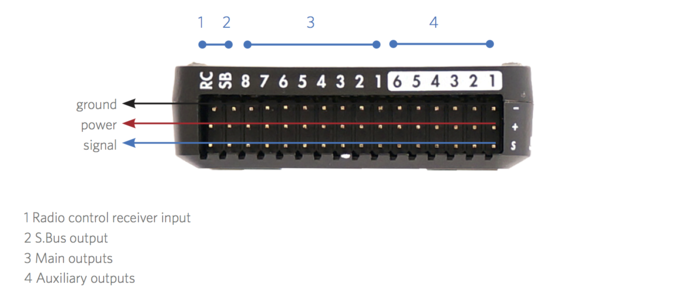
\includegraphics[width=1.0\textwidth]{figures/pixhawk_outputs}
  \caption{Pixhawk outputs for servos. Image from
    \url{http://copter.ardupilot.com/wiki/common-autopilots/common-pixhawk-overview/}.}
  \label{fig:pixhawk_outputs}                                                              
\end{figure}

AUX OUT 5-6 are, by default, set up as relays. The number of AUX OUT
ports set up as servo outputs can be changed in Mission Planner with
the \texttt{BRD\textunderscore PWM\textunderscore COUNT} parameter, in
the way that setting \texttt{BRD\textunderscore PWM\textunderscore
 COUNT} to 6 gives servo output on AUX OUT 1-6.

The IRIS$^+$ transmitter and receiver has eight channels. This is
reflected in the way that a vector of eight components can be sent to
the quad via the topic /irisX/mavros/rc/override/. The first four
components are for roll, pitch, throttle and yaw, leaving the other
four for servos. In addition to that, the different channels needs to
be connected to the different servo outputs on the Pixhawk. This can
be done in the Mission Planner. In Mission Planner, the eight channels
are named RC1-RC8. The different servo ports are named in a similar
way: RC1-RC8 corresponds to MAIN OUT 1-8 and RC9-RC14 corresponds to
AUX OUT 1-6. Unfortunately, in the current version of Mission Planner,
there is no general way of connecting channel RCX to RCY, X $= 1 \dots
8$, Y = $= 1 \dots 14$. If three or less servos are needed, the built
in settings for a camera gimbal can be used.\footnote{Which signals to
be sent to which servo output are controlled by the parameter
\texttt{RCX\textunderscore FUNCTION}, X $= 1 \dots 14$, in Mission
Planner. For these parameters, there is an option called
\texttt{Passthrough}, passing channel X to output X, but since there
are eight channels, only MAIN OUT 1-8 can be reached by this option,
not AUX OUT 1-6.}

The Pixhawk does not provide power to the servos itself, so these must
be powered in other ways. A BEC or ESC, providing 5 V, can be used,
for example. It can be connected to the servo outputs on the Pixhawk
or to the servo directly. By default, the ground pins are connected to
the ground of the battery, by a wire to MAIN OUT 1 ground pin. Also,
on the bottom of the IRIS$^+$ there are a black cable connected to AUX
OUT 6 ground pin and a white cable connected to AUX OUT 1 signal
pin. In addition to this, there is a red power cable and another black
ground wire connected to the battery of the IRIS$^+$, providing 12
V. So, if the voltage is lowered to around 5 V this can be used. So if
only one servo is needed, the quadcopter does not even needs to be
opened!

For additional tips and tricks, see
\url{http://copter.ardupilot.com/wiki/common-optional-hardware/common-servo/}
and \url{https://learn.adafruit.com/quadcopter-spray-can-mod/}. A
wiring diagram for the Pixhawk can be found in
\url{http://copter.ardupilot.com/wiki/advanced-pixhawk-quadcopter-wiring-chart/}.


\end{document}
